\chapter{Antecedentes}
\label{chap:antecedentes}

\drop{E}{n} este capitulo se hace una introducción a los aspectos más destacables relacionados con
el \acs{TFG}. Se empieza presentando el concepto de interacción implícita. Después se ponen en
contexto los sistemas de navegación por satélite y sus actuales aplicaciones para smartphone. Más
tarde se hace un estudio por las principales plataformas de desarrollo. Luego se
indaga en el concepto de wearable y se describen los diferentes tipos de wearable en función de la
forma de conectarse con el teléfono. Finalmente se hace un repaso por los principales proveedores de
servicios que serán necesarios a la hora de implementar nuestro sistema.

Con todo ello se espera adquirir los conocimientos necesarios para desarrollar el \acs{TFG}.

\section{Interacción implícita}

Baecker y Buxton definieron en 1987 la \acf{IPO} como «todos los intercambios que suceden entre la
  persona y el ordenador». En el modelo clásico de \acs{IPO} es la persona la encargada de
interactuar con el ordenador y decirle qué hacer, es decir, interacción explícita. Pero hay otra
forma de proceder: que sea el ordenador el encargado de interactuar con la persona sin a intención
explícita o el conocimiento del usuario, es decir, interacción implícita.

En base a ello, podemos definir la interacción implícita como un tipo \acs{IPO} en el que la
computadora es la encargada de interactuar con el usuario.

En este \acs{TFG} se hará uso de la interacción implícita por medio de la vibración y el sonido para
comunicarnos con el usuario en los momentos necesarios y decirle qué acción ha de realizar. Otros
proyectos que utilizan este tipo de interacción para el guiado de personas son \cite{Boemo12} y
\cite{Merino13}, o las zapatillas \textit{Lechal} \cite{Lechal}.

\section{Sistemas de navegación por satélite}

Un \acs{SGNS} o \acs{GNSS} consiste en una constelación de satélites que transmite señales que
permiten determinar nuestras coordenadas geográficas, la altitud y la hora (cuatro dimensiones) con
mucha exactitud, en cualquier parte del mundo, las 24 horas y en todas las condiciones
climatológicas.

El origen de la navegación por satélite se remonta a los años sesenta cuando el ejército de Estados
Unidos desarrolló Transit basado en el efecto Doppler~\cite{SN}. Los satélites viajaban por caminos
conocidos y transmitiendo una frecuencia conocida. La frecuencia recibida difería ligeramente de la
frecuencia de emisión debido al movimiento del satélite. Mediante dicha variación, el receptor puede
determinar su ubicación a un lado o al otro del satélite, y varias de estas mediciones combinadas
con un conocimiento preciso de la órbita del satélite pueden determinar una posición el
particular. Este sistema requería que el receptor estuviera casi estático unos 40 minutos para
establecer su posición.

La primera vez que apareció el concepto de \acs{SGNS} para guiar a civiles fue en 1983 cuando Honda
se planteó utilizar esta tecnología y desarrolló su sistema de navegación para coches. Pero no lo
culminó hasta 1990 cuando lo integró en el Honda Legend Acura Legend~\cite{Parra13}.

El funcionamiento de los \acs{SGNS} modernos es más directo. El satélite emite una señal que
contiene los datos orbitales necesarios para calcular su posición y el tiempo preciso en el que se
transmitió la señal. De este modo, el receptor compara el momento de la emisión con el tiempo de
recepción y puede establecer su posición con respecto al satélite. Y, al utilizar varios satélites
podremos establecer nuestra posición el globo mediante la trilateración (ver
figura~\ref{fig:trilateracion}).

\begin{figure}[!h]
  \begin{center}
    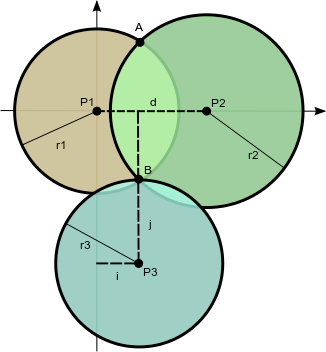
\includegraphics[width=0.5\textwidth]{/trilateracion.png}
    \caption{Ejemplo de trilateración. Estando en B, queremos conocer su posición relativa a los
      puntos de referencia P1, P2, y P3 en un plano bidimensional. Al medir r1 se reduce nuestra
      posición a una circunferencia. A continuación, midiendo r2, la reducimos a dos puntos, A y
      B. Una tercera medición, r3, nos devuelve nuestras coordenadas en B. Una cuarta medición
      también puede hacerse para reducir y estimar el error.}
    \label{fig:trilateracion}
  \end{center}
\end{figure}

\subsection{Coordenadas geográficas}

Las coordenadas geográficas son el sistema que nos permite representar nuestra posición el
globo. Este sistema de referencia hace uso de dos coordenadas angulares latitud (Norte y Sur) y
longitud (Este y Oeste) medidas desde el centro de la tierra y expresadas por regla general en
grados sexagesimales.

\begin{itemize}
  \item La latitud es el ángulo que forma el Ecuador con el punto que medimos.
  \item La longitud es el ángulo se forma entre el meridiano de Greenwich con el punto que medimos.
\end{itemize}

\subsection{Tecnologías actuales}

En la actualidad predominan dos tecnologías: \acf{GPS} y \acf{GLONASS}. En los siguientes apartados
se resumen sus características más importantes.

No se han incluido en el estudio ninguno de los sistemas que a fecha de hoy no se consideran
operativos~\cite{SPSA} como:

\begin{itemize}
  \item Galileo desarrollado por la Unión Europea.
  \item \acf{BNTS} desarrollado por la República Popular de China.
  \item \acf{QZSS} desarrollado por Japón.
  \item \acf{IRNSS} desarrollado por India.
\end{itemize}

\begin{definitionlist}
  \item[\acf{NAVSTAR-GPS}] Este sistema, también conocido simplemente por \acs{GPS} es el sistema
    de navegación desarrollado por los Estados Unidos. Los primeros proyectos relacionados empezaron
    a desarrollarse en 1973 y en ellos se establecieron las bases de lo que hoy conocemos como
    \acs{GPS}. Los primeros satélites se lanzaron en 1978 y el programa fue plenamente operativo en
    1995, aunque con un sistema de degradación de señal para los usos civiles que limitaba la señal
    a una precisión aleatoria entre 15 y 100 metros. En mayo del año 2000 se eliminó dicha
    limitación permitiendo determinar la posición y la hora de forma precisa, con un error nominal
    de unos 15 metros.

    En la actualidad, esta tecnología es accesible por la mayoría de los smartphones. Está formada
    por una constelación de 24 a 27 satélites que se mueven en órbita de unos 20.000 km, por seis
    planos y con una inclinación de 55 grados.

  \item[GLONASS] Al mismo tiempo que se desarrollaba el \acs{GPS}, los rusos también desarrollaron
    su sistema de navegación \acs{GLONASS}. Los primeros satélites fueron lanzados en 1982 pero el
    programa no fue operativo hasta 1996 con unos 9 a 11 satélites y un sistema de degradación de
    señal para usos civiles parecido al de \acs{GPS}. Esta limitación hacía que la precisión fuese
    de unos 30 metros. En 2007 se eliminaron las limitaciones para uso civil y en 2012 se convirtió
    en un sistema de navegación plenamente funcional cuando se pusieron en órbita más satélites. El
    sistema \acs{GLONASS} está optimizado para ser usado en el hemisferio norte y proporciona la
    posición con un error entre 5 y 15 metros.

    En la actualidad, esta tecnología puede ser usada sólo por algunos smartphones. Está formada por
    una constelación de 31 satélites que orbitan a una altitud de 19.100 km, situados en tres planos
    y con una inclinación de 64,8 grados.

\end{definitionlist}


\subsection{Aplicaciones de navegación para smartphone}

Aunque existen una gran cantidad de aplicaciones de navegación para smartphone disponibles en las
tiendas oficiales de aplicaciones, en este apartado analizaremos solamente las aplicaciones más
usadas.

\begin{definitionlist}
  \item[Google maps] Google Maps es una aplicación de navegación lanzada por Google en Septiembre de
    2008 que se puede utilizar tanto en Android como en iOS, Windows Mobile, Symbian o
    BlackBerry. Además, Google Maps está disponible en múltiples lenguajes.

    Entre las características de la aplicación de Google podemos destacar las siguientes:

    \begin{itemize}
      \item Visualización de nuestra posición el mapa mostrando el posible error cometido en la
        trilateración.
      \item Visualización de mapas offline previamente descargados.
      \item Visualización de la cantidad e tráfico de las carreteras.
      \item Visualización de edificios en 3D en algunas ciudades.
      \item «Street View» o posibilidad de ver las calles como si te encontrases en ellas.
      \item Rotación automática del mapa en función de nuestra orientación.
      \item Cálculo de rutas para peatones, transporte público y vehículos motorizados.
    \end{itemize}

    Las interacciones que utiliza Google Maps para comunicarse con el usuario se realizan por medio
    de la pantalla, el sonido y la vibración. La pantalla muestra continuamente las próximas
    acciones a realizar y, cuando se estima oportuno, el smartphone vibra y se escucha por los
    altavoces la instrucción a realizar. La vibración que se utiliza es la misma para todos los
    tipos de instrucciones.

  \item[iOS maps] iOS Maps es la aplicación de Apple lanzada en Septiembre de 2012 para sus
    dispositivos iPhone, iPad y iPod Touch. Esta aplicación es multilenguaje.

    Entre sus características podemos destacar:

    \begin{itemize}
      \item Visualización de nuestra posición el mapa mostrando el posible error cometido en la
        trilateración.
      \item Visualización de la cantidad e tráfico de las carreteras.
      \item Visualización de edificios en 3D en algunas ciudades.
      \item Rotación automática del mapa en función de nuestra orientación.
      \item Cálculo de rutas para peatones y vehículos motorizados.
    \end{itemize}

    Con respecto a la interacción con el usuario, iOS maps utiliza la pantalla y el sonido. La
    pantalla mostrando continuamente las instrucciones a seguir y el sonido a la hora de realizar
    las instrucciones.

  \item[Nokia HERE] Nokia HERE, antes conocido como Ovi Maps (2007-2011) y como Nokia Maps
    (2011-2012), es la aplicación de navegación desarrollada por Nokia. Está disponible para Windows
    Phone, Symbian y Android; y está disponible en múltiples lenguajes.

    Entre sus características es importante destacar:

    \begin{itemize}
      \item Visualización de nuestra posición el mapa mostrando el posible error cometido en la
        trilateración.
      \item Visualización de mapas offline previamente descargados.
      \item Visualización de la cantidad e tráfico de las carreteras.
      \item Visualización de edificios en 3D en algunas ciudades.
      \item Rotación automática del mapa en función de nuestra orientación.
      \item Cálculo de rutas para peatones, transporte público y vehículos motorizados.
    \end{itemize}

    Con respecto a la interacción con el usuario, HERE utiliza la pantalla y el sonido. La
    pantalla mostrando continuamente las instrucciones a desarrollar y, a la hora de realizar
    las instrucciones, se reproducen sonoramente.

  \item[OsmAnd] OsmAnd es la aplicación de navegación de código abierto (GPL v3) para Android basada
    en los mapas de \acf{OSM}. Existe una versión gratuita y otra de pago que nos permite
    desbloquear el limite de descargas de mapas offline y ayudar al desarrollo de la aplicación.

    Entre las características más importantes podemos destacar:

    \begin{itemize}
      \item Visualización de nuestra posición el mapa mostrando el posible error cometido en la
        trilateración.
      \item Visualización de mapas offline previamente descargados.
      \item Rotación automática del mapa en función de nuestra orientación.
      \item Cálculo de rutas para peatones y vehículos motorizados.
    \end{itemize}

    La interacción con el usuario se realiza visualizando la pantalla (que puede configurarse para
    que se encienda antes de cada acción) y por medio del sonido.

\end{definitionlist}

\section{Plataformas smartphone}

Dese la aparición de la industria dedicada a la telefonía móvil allá por 1983 cuando la compañía
Motorola estrenó el primer móvil de la historia, el Motorola DynaTAC 8000X, se han sucedido una
serie de mejoras continuas hasta ofrecer al usuario la posibilidad de estar continuamente conectado
para llegar a lo que hoy conocemos como smartphone

El éxito de los teléfonos inteligentes o smartphones radica en que ofrecen la posibilidad de llevar
continuamente con nosotros un ordenador en el que se pueden instalar multitud de aplicaciones. Estos
programas tienen finalidades muy dispares, desde aplicaciones relacionadas con el ámbito laboral
como gestores de correo electrónico y editores de texto, hasta aplicaciones de ocio como juegos y
redes sociales.

A lo largo de estos años, los fabricantes se han basado en diferentes \acf{SO} especialmente
diseñados para la telefonía móvil a la hora de gestionar los terminales. Estos \acs{SO} están
enfocados en exprimir las capacidades multimedia e inalámbricas de los dispositivos.

Puesto que cada sistema cuenta con sus propias aplicaciones, los \acs{SO} han ido adquiriendo mayor
importancia de forma que existe una guerra por hacerse por la mayor cuota de mercado.

Este \acs{TFG} pretende aprovechar la popularidad de los smartphone para hacer llegar nuestra
aplicación al mayor número de usuarios. Para ello, tendremos que decidir cuál será la plataforma
sobre la que se desarrollará el proyecto: Android, iOs, Windows Phone o Blackberry.

A pesar de que Symbian de Nokia tenía bastante popularidad hace no demasiados años, queda
completamente descartado del estudio porque en la actualidad posee menos del 0.5\% de cuota de
mercado y está previsto dejar de implantarlo en nuevos terminales a partir de
2016~\cite{Litchfield13}.

\subsection{Android}

Andorid es un \acs{SO} basado en Linux desarrollado por la Open Handset Alliance liderada por
Google. Su lanzamiento tuvo lugar en Octubre de 2008 y, desde entonces, se ha hecho con el
81\%~\cite{Llamas13} de la cuota de mercado de los smartphones. La última versión de este \acs{SO}
 es la 5.0.1 o «Lollipop» y el lenguaje de programación de aplicaciones es Java.

Uno de las principales causas de su éxito es ser un sistema abierto. Esto ha permitido que salgan al
mercado una gran multitud de terminales con características y precios muy distintos que han
conseguido que llegue a la mayoría de los usuarios de smartphone.

\begin{definitionlist}
  \item[Ventajas] Android cuenta con la mayor cuota de mercado y facilidad a la hora de empezar a
    desarrollar y posteriormente probar la aplicación. Además, para distribuir la aplicación por
    medio de la tienda oficial, la Play Store, sólo hay que pagar previamente 25\$.

    Por otro lado, gracias a la variedad de fabricantes, Android posee una gran variedad de
    dispositivos con diferentes características y podremos seleccionar el dispositivo con la
    potencia y características que necesitemos.

  \item[Desventajas] Las principales ventajas también suponen algunos problemas. El hecho de que
    haya diferentes dispositivos con diferente hardware nos complica garantizar el rendimiento
    óptimo de nuestra aplicación en las diferentes configuraciones de pantalla, memoria y
    procesador.

\end{definitionlist}

\subsection{iOS}

Es el \acs{SO} desarrollado por Apple para iPhone aunque posteriormente se portó para otros
dispositivos de la compañía como iPad o iPod Touch. Su lanzamiento tuvo lugar en Junio de 2007 junto
con el primer iPhone y en la actualidad cuenta con un 12.9\%~\cite{Llamas13} de la cuota de
mercado. La última versión de este \acs{SO} es la 8.1.2 y el lenguaje de programación de
aplicaciones es Objetive-C.

Apple iOS ha sido durante mucho tiempo la referencia de los desarrolladores de aplicaciones ya que
fue el primero en incorporar una tienda de aplicaciones: AppStore. Con ello, permitió desarrollar a
terceros aplicaciones para sus dispositivos y mantenerlas bajo el control de Apple.

\begin{definitionlist}
  \item[Ventajas] Puesto que el \acs{SO} está diseñado específicamente para una configuración de
    hardware, iOS permite explotar al máximo sus capacidades y desarrollar aplicaciones para un
    pequeño grupo de dispositivos bastante potentes.

  \item[Desventajas] Apple no permite instalar de forma legal aplicaciones que no hayan sido
    validadas por medio de su AppStore. Si queremos desarrollar aplicaciones deberemos pagar una
    licencia anual de 99\$.

    Por otro lado, los dispositivos de Apple son en general bastante caros y no están al alcance de
    todo el mundo.

\end{definitionlist}

\subsection{Windows Phone}

Es el \acs{SO} desarrollado por Microsoft sucesor de Microsoft Mobile y llamado originalmente Pocket
PC. Fue presentado en 2010 y en la actualidad cuenta con el 3.7\%~\cite{Llamas13} de la cuota de
mercado. La última versión del \acs{SO} es la 8.1 y soporta los lenguajes programación C\# y Visual
Basic .NET.

En 2011 se anunció una alianza con Nokia por la cual se convertirá en el principal \acs{SO} de la
compañía finlandesa. Por ello, a partir de 2016 los teléfonos que antaño utilizaban Symbian
utilizarán Windows Phone.

\begin{definitionlist}
  \item[Ventajas] Microsoft provee de un entorno de trabajo como Visual Studio, con una gran
    cantidad de \acf{API}, que permite que la programación resulte lo más sencilla posible.

  \item[Desventajas] La mayor desventaja de Windows Phone viene dada por su tardía llegada al
    mercado que le ha hecho difícil competir con los otros \acs{SO}. Estos ya tienen bastante cuota
    de mercado y, al no ofrecer grandes saltos de calidad, no ha podido convencer a los usuarios.

    Por otro lado, para publicar aplicaciones en la tienda oficial, es necesario pagar una licencia
    de 75\euro{}.

\end{definitionlist}

\subsection{Blackberry}

Blackberry es un \acs{SO} desarrollado por la empresa canadiense Research In Motion. Tuvo sus
inicios en 1999 incorporando funciones típicas hoy en día como acceso al correo electrónico e
Internet. En la actualidad tiene un 1.7\%~\cite{Llamas13} de cuota de mercado. La última versión de
este \acs{SO} es Blackberry 10 y el lenguaje de programación de las aplicaciones es Java.

Aunque este sistema está orientado especialmente a empresas y profesionales, tuvo un gran éxito
entre los jóvenes gracias a su servicio de mensajería instantánea.

\begin{definitionlist}
  \item[Ventajas] No es necesario pagar para subir aplicaciones a su tienda oficial de aplicaciones
    llamada App World. Sólo es necesario registrarnos como desarrollador y que aprueben nuestra
    aplicación.

    Para determinados tipos de usuario puede considerarse una ventaja que la mayoría de terminales
    dispongan de un teclado físico.

  \item[Desventajas] De igual modo, disponer de un teclado físico limita las posibilidades de
    desarrollo frente a dispositivos con pantallas táctiles.

    Además, su tienda de aplicaciones cuenta con poco apoyo por parte de los desarrolladores y, en
    consecuencia, dispone de muchas menos aplicaciones que la competencia.

\end{definitionlist}

\section{Wearables}

La palabra wearable hace referencia al conjunto de aparatos y dispositivos que se sitúan en alguna
parte del cuerpo interactuando continuamente con el usuario y con otros dispositivos para realizar
alguna función específica. Hoy en día podemos encontrar relojes, pulseras, colgantes, anillos,
gafas, ropa o zapatillas que cumplen con esta descripción.

El término wearable tiene raíz inglesa y se puede traducir como «llevable» o «vestible» haciendo
referencia a computadoras corporales o «llevables» por el usuario. Bajo esta visión, el ordenador
deja de ser un elemento externo al usuario que usa en determinados espacios para convertirse en un
elemento con el que interactúa continuamente y lo lleva a todos sitios.

Dentro de esta definición no se considera wearable a otros elementos que usamos diariamente como la
televisión, la cafetera o nuestro lector de ebooks pese a llevar procesadores. Esto es así porque no
forman parte de nosotros, es decir, no son «llevables» o «vestibles».

Se estima que los orígenes de la tecnología wearable data de la década de 1970 pero no ha sido hasta
la década del 2010 cuando la tecnología ha evolucionado lo suficiente para atraer a los
consumidores. 

Las grandes compañías están apostando por la tecnologías wearables.  En la
\acf{CES}\footnote{http://www.cesweb.org/} de enero de este año, grandes empresas como Intel,
Adidas, Sony o Rebook han presentado diferentes complementos wearables. Más tarde, en abril, Google
presentó sus Google Glass y se espera la llegada del AppleWatch de Apple para la primavera de
2015. Todo ello hace pensar que los wearables han llegado para quedarse y que los próximos años
sufrirán una gran expansión.

En este \acs{TFG} se pretende aprovechar la creciente popularidad de los wearables utilizando alguno
del mercado como complemento vibratorio. De esta forma conseguiremos que nuestro sistema final pueda
ser usado por la mayor cantidad de gente posible.

\subsection{Wearables vibratorios para smartphone}

A pesar de la gran variedad de dispositivos wearables, no todos tienen la misma forma de interacción
con el usuario y en este \acs{TFG} sólo estamos interesados en los que se puedan sincronizar con un
smartphone y sean vibratorios.

A continuación se habla de los diferentes tipos de wearables que disponen de vibración separándolos
por la forma que tienen de conectarse con el smartphone.

\begin{definitionlist}
  \item[Perfiles bluetooth] La mayoría de dispositivos de bajo coste como colgantes, anillos o
    pulseras utilizan este método de conexión con el smartphone. Básicamente se sincronizan con
    nuestro móvil con el perfil de manos libres o \acf{HFP} para que cuando recibamos una llamada
    el wearable vibre. Como consecuencia de ello, resulta imposible desarrollar aplicaciones para
    estos complementos porque no podemos controlar a voluntad la vibración del wearable y, de
    hacerlo vibrar simulando una llamada, no podríamos diferenciar entre una llamada real o una
    simulada.

  \item[Bluetooth con aplicación propietaria] Otros dispositivos como pulseras o relojes se
    sincronizan con nuestro smartphone por medio de bluetooth y sus perfiles \acf{HID} o
    \acf{PAN}. Gracias a ello pueden comunicarse con la aplicación propietaria instalada en el
    smartphone, configurar los wearables y recibir la información almacenada en el dispositivo.

    Este tipo conexión es bastante común en los cuantificadores personales pero, al tratarse de
    software propietario, es necesaria una \acs{API} para poder realizar aplicaciones para
    ellos. Sorprendentemente sólo la empresa Fitbit proporciona una
    \acs{API}\footnote{http://dev.fitbit.com/} pero no permiten manipular el vibrador de su
    dispositivo.

  \item[Bluetooth con Google Play services] Este tipo de conexión es la que realizan los wearables
    que utilizan como \acs{SO} Android Wear para comunicarse con el smartphone Android. Esto permite
    que las notificaciones del smartphone lleguen a nuestro wearable de forma transparente al
    desarrollador y se instalen aplicaciones en el wearable por medio del smartphone.

    A pesar de que Android Wear fue lanzado por Google en marzo de 2014 se trata de una plataforma
    de desarrollo muy potente porque incorpora la mayoría de la \acs{API} de
    Android~\cite{APIAW}. Gracias a ello, se puede controlar el vibrador del wearable a voluntad.
 
\end{definitionlist}

\section{Proveedores de mapas, rutas y geocoding}

Para la realización en este \acs{TFG} del sistema de guiado por satélite será necesario utilizar
alguno de los proveedores de mapas rutas y geocoding. A continuación se muestran principales
proveedores de estos servicios. Sobra decir que, salvo restricciones de licencia, es posible
utilizar los servicios de forma combinada.

\begin{definitionlist}
  \item[Google] Google es el proveedor de mapas, rutas y geocoding más conocido de la
    actualidad. Aunque ofrece los tres servicios como servicios web accesibles por medio de
    \acs{API} y están disponibles para todas las plataformas, poseen una gran integración con
    Android.

    Por un lado, la \acs{API} de mapas permite insertar mapas de todas las partes del mundo con el
    logotipo de Google en nuestra aplicación. De forma gratuita podemos realizar hasta
    2.500~\cite{LicenciaAndroid} solicitudes de mapas con 25.000 muestras y con una resolución de
    640 x 640.

    Por otro, el servicio de rutas nos permite calcular hasta 2.500 rutas diferentes con hasta 10
    hitos por solicitud. Este servicio nos permite diferenciar entre rutas para peatones, ciclistas,
    vehículos motorizados o transporte público.

    Finalmente, el servicio de geocoding de Google permite realizar gratuitamente hasta 2.500
    peticiones al día. Además, se pueden realizar búsquedas por números de casa.

  \item[Bing] Es el proveedor de mapas de Microsoft que proporciona una \acs{API} con interface
    \acf{REST} para integrar los servicios de mapas, geocoding y rutas en cualquier aplicación.

    Tanto si la aplicación que desarrollemos está disponible para la descarga gratuita como si es de
    pago, Bing nos permite un máximo de 125.000~\cite{LicenciaMicrosoft} transacciones por año
    gratuitamente. En estas peticiones van incluidos todos los servicios.

  \item[HERE] Es un proveedor de mapas, rutas y geocoding de Nokia que dispone de \acf{SDK} para el
    desarrollo de aplicaciones en iOS y Android.

    HERE permite realizar un total de 100.000~\cite{LicenciaHERE} peticiones gratuitas al mes entre
    imágenes de satélite, geocoding y rutas. Es necesario destacar que sólo se pueden calcular rutas
    para vehículos motorizados y personas, y que la versión de geocoding gratuita no permite buscar
    a al nivel de números de casa.

  \item[Open Street Map] \acs{OSM} es un proyecto colaborativo para crear mapas libres y
    gratuitos. Por ello, es posible utilizar sus mapas y rutas bajo la licencia
    ODbL~\cite{LicenciaOSM}.

    Su servicio de rutas permite la opción de calcularlas para peatones, ciclistas y vehículos
    motorizados. Para ello es necesario registrarse gratuitamente y obtener una clave de usuario.

    Por otro lado, el servicio de geocoding de \acs{OSM} se llama Nominatim y funciona sobre
    servidores mantenidos por medio de donaciones y con una capacidad limitada. Por ello, dicen
    poner el límite en «un máximo absoluto de 1 petición»~\cite{Nominatim} aunque es posible
    realizar varias. Este servicio no permite realizar búsquedas a nivel de números de casa.
 
\end{definitionlist}

% Local Variables:
% TeX-master: "main.tex"
%  coding: utf-8
%  mode: latex
%  mode: flyspell
%  ispell-local-dictionary: "castellano8"
% End:
